\chapter{从开弦量子到快子与引力}

\lectureoverview{我们现在对上一讲中得到的简正模进行量子化，并追问它们产生什么样的粒子态。每个横向模都是一个谐振子，但其归一化略显陌生：激发第\(n\)模会使光前能量、从而质量平方能级升高\(n\)个单位。开弦的第一激发能级的变换性质恰好与无质量矢量的两个横向极化相同。因此，相对论一致性要求基态质量平方为负。该态就是玻色弦快子，其真正意义在于真空不稳定，而不是一种实际可用的超光速粒子。最后，一旦弦发生相互作用，弦的合并与分裂使得闭弦不可避免；最低的闭弦激发将成为引力子。}

\section{隐藏在每个弦模中的谐振子}

对于一个横向坐标\(X\)，第\(n\)个非零简正模具有能量和拉格朗日量

\begin{align}
  E_n
  &=
  \frac14\dot X_n^{\,2}
  +\frac{n^2}{4}X_n^2,
  \label{eq:l03-mode-energy}\\
  L_n
  &=
  \frac14\dot X_n^{\,2}
  -\frac{n^2}{4}X_n^2.
  \label{eq:l03-mode-lagrangian}
\end{align}

\(1/4\)的因子并非错误。它们记录了将弦作用量约化为独立傅里叶模时所选择的归一化。因此，构造哈密顿量的第一步是计算正则动量，

\begin{equation}
  p_n=\frac{\partial L_n}{\partial\dot X_n}
     =\frac12\dot X_n,
  \qquad
  \dot X_n=2p_n.
  \label{eq:l03-canonical-momentum}
\end{equation}

勒让德变换给出

\begin{equation}
  H_n=p_n\dot X_n-L_n
     =p_n^2+\frac{n^2}{4}X_n^2.
  \label{eq:l03-mode-hamiltonian}
\end{equation}

\begin{figure}[H]
  \centering
  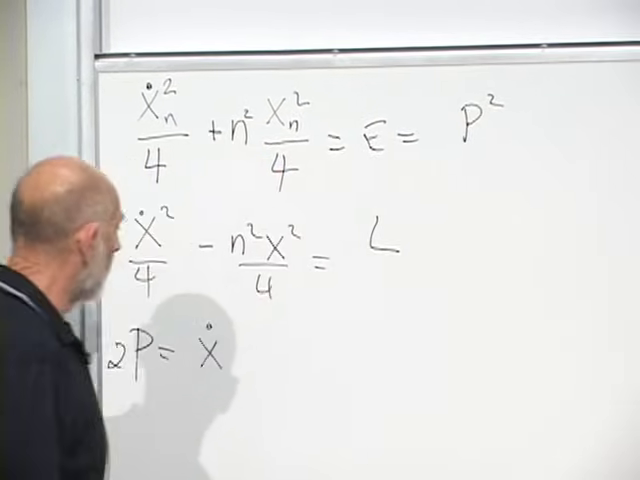
\includegraphics[width=0.82\textwidth]{lecture_03_figure_01.png}
  \caption{在从开弦继承的归一化下，模能量、拉格朗日量、正则动量与哈密顿量。}
  \lectureframe{00:05:40}
  \label{fig:l03-mode-hamiltonian-board}
\end{figure}

为了将\(H_n\)因式分解，把\(X_n\)与\(p_n\)组合为

\begin{equation}
  \frac{nX_n}{2}\pm i p_n.
\end{equation}

经典地，这两个因子会对易，但量子力学地

\begin{equation}
  [X_n,p_m]=i\delta_{nm}
  \label{eq:l03-canonical-commutator}
\end{equation}

在以\(\hbar=1\)为单位的条件下。交叉项并不会无害地相消。对于一个固定模，

\begin{align}
  \left[\frac{nX_n}{2}+ip_n,
        \frac{nX_n}{2}-ip_n\right]
  &=n,
  \label{eq:l03-unscaled-commutator}\\
  \left(\frac{nX_n}{2}-ip_n\right)
  \left(\frac{nX_n}{2}+ip_n\right)
  &=H_n-\frac n2.
  \label{eq:l03-factorized-hamiltonian}
\end{align}

\begin{figure}[H]
  \centering
  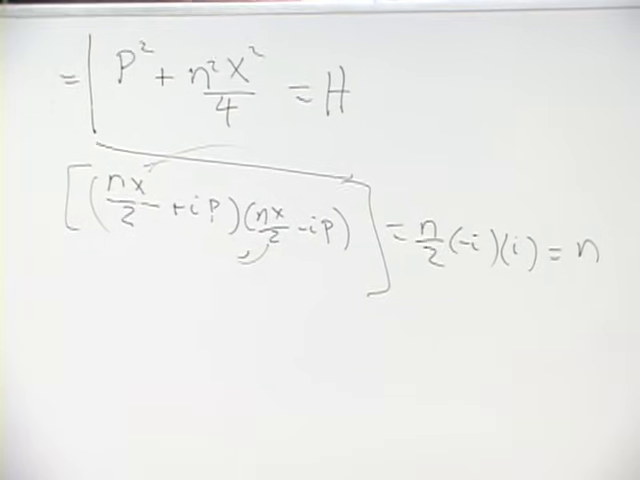
\includegraphics[width=0.82\textwidth]{lecture_03_figure_02.png}
  \caption{黑板计算中，正则对易子提供了\(n\)的因子。}
  \lectureframe{00:10:30}
  \label{fig:l03-commutator-board}
\end{figure}

\(n\)的因子告诉我们如何归一化升降算符：

\begin{align}
  a_n
  &\equiv
  \frac{\sqrt n}{2}X_n+\frac{i}{\sqrt n}p_n,
  \label{eq:l03-annihilator}\\
  a_n^\dagger
  &\equiv
  \frac{\sqrt n}{2}X_n-\frac{i}{\sqrt n}p_n.
  \label{eq:l03-creator}
\end{align}

它们满足

\begin{equation}
  [a_n,a_m^\dagger]=\delta_{nm},
  \qquad
  H_n=n\left(a_n^\dagger a_n+\frac12\right).
  \label{eq:l03-oscillator-algebra}
\end{equation}

因此，\(a_n^\dagger\)增加第\(n\)个谐振子的一个量子，但该量子携带\(n\)个单位的模能量。熟悉的谐振子间距并未丢失；其频率为\(\omega_n=n\)。

\begin{figure}[H]
  \centering
  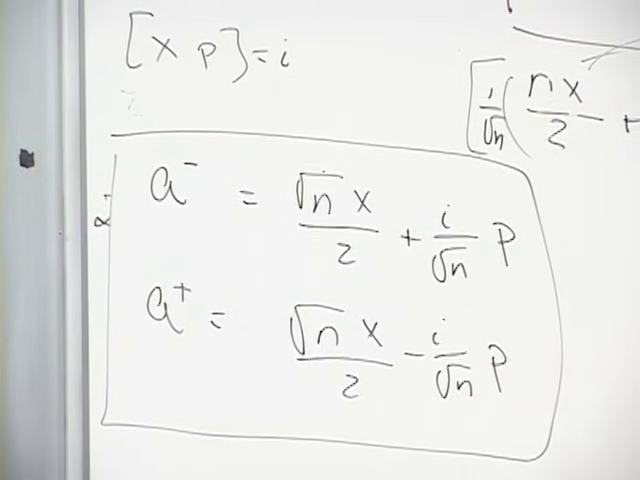
\includegraphics[width=0.82\textwidth]{lecture_03_figure_03.png}
  \caption{第\(n\)个弦谐振子的归一化湮灭算符与产生算符。}
  \lectureframe{00:12:00}
  \label{fig:l03-ladder-board}
\end{figure}

\subsection{两座横向振子塔}

在四维时空中，一根沿\(z\)轴携带极大动量的弦有两个横向坐标，\(X\)和\(Y\)。因此我们需要两座独立的振子塔。令\(a_n,a_n^\dagger\)作用于\(X\)模，\(b_n,b_n^\dagger\)作用于\(Y\)模。由\eqref{eq:l03-annihilator}--\eqref{eq:l03-creator}解出坐标，得到

\begin{equation}
  X_n=\frac{a_n+a_n^\dagger}{\sqrt n},
  \qquad
  Y_n=\frac{b_n+b_n^\dagger}{\sqrt n}.
  \label{eq:l03-mode-coordinates}
\end{equation}

\begin{figure}[H]
  \centering
  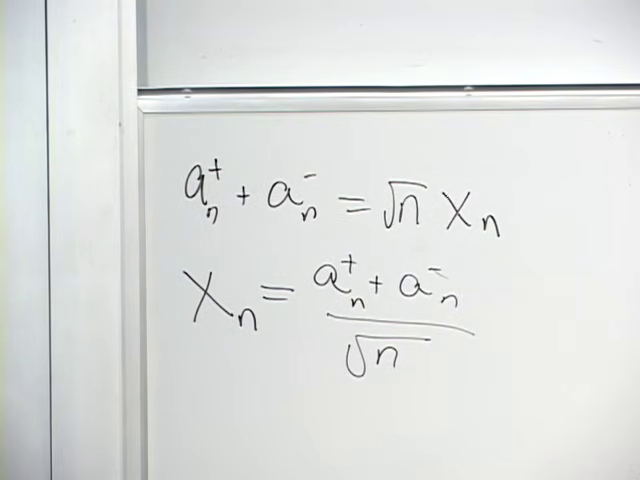
\includegraphics[width=0.78\textwidth]{lecture_03_figure_04.png}
  \caption{用产生算符与湮灭算符解出模坐标。}
  \lectureframe{00:17:05}
  \label{fig:l03-coordinate-operator-board}
\end{figure}

开弦坐标按诺伊曼模展开，

\begin{align}
  X(\sigma,\tau)
  &=X_{\rm cm}(\tau)
    +\sum_{n=1}^{\infty}X_n(\tau)\cos(n\sigma),
  \label{eq:l03-X-fourier}\\
  Y(\sigma,\tau)
  &=Y_{\rm cm}(\tau)
    +\sum_{n=1}^{\infty}Y_n(\tau)\cos(n\sigma).
  \label{eq:l03-Y-fourier}
\end{align}

出现余弦是因为端点斜率消失。代入\eqref{eq:l03-mode-coordinates}使弦本身成为一个算符：

\begin{align}
  X(\sigma,\tau)
  &=X_{\rm cm}(\tau)
    +\sum_{n=1}^{\infty}
      \frac{a_n(\tau)+a_n^\dagger(\tau)}{\sqrt n}
      \cos(n\sigma),
  \label{eq:l03-X-operator}\\
  Y(\sigma,\tau)
  &=Y_{\rm cm}(\tau)
    +\sum_{n=1}^{\infty}
      \frac{b_n(\tau)+b_n^\dagger(\tau)}{\sqrt n}
      \cos(n\sigma).
  \label{eq:l03-Y-operator}
\end{align}

\begin{figure}[H]
  \centering
  \begin{minipage}[t]{0.48\textwidth}
    \centering
    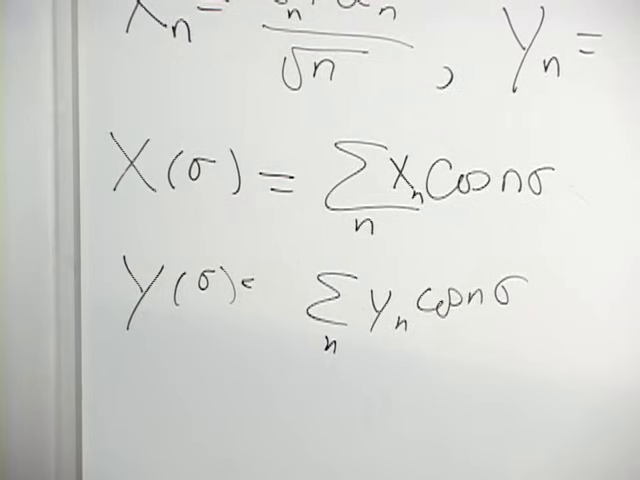
\includegraphics[width=\textwidth]{lecture_03_figure_05.png}
    \par\smallskip\footnotesize (a) 坐标模展开。
  \end{minipage}\hfill
  \begin{minipage}[t]{0.48\textwidth}
    \centering
    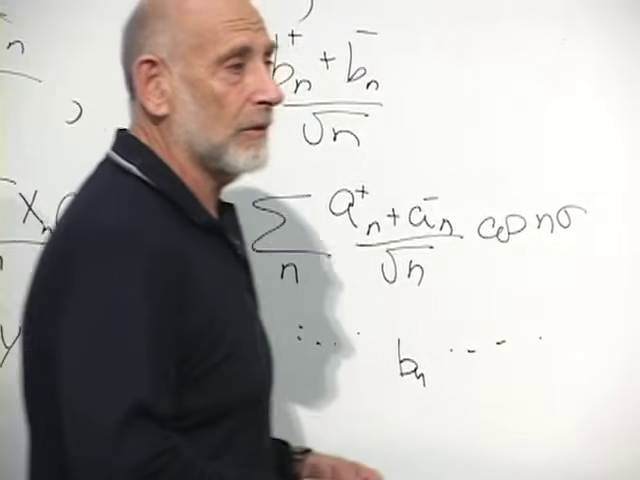
\includegraphics[width=\textwidth]{lecture_03_figure_06.png}
    \par\smallskip\footnotesize (b) 将升降算符代入弦坐标。
  \end{minipage}
  \caption{量子开弦的形状由其所有横向振子算符组装而成。}
  \lectureframe{00:20:35 and 00:21:05}
  \label{fig:l03-string-coordinate-board}
\end{figure}

\begin{classroomqa}
\audiencequestion{\(X_n\)也是\(\sigma\)的函数吗？\lecturetimestamp{00:21:48}}
\lecturerresponse{不是。对\(\sigma\)的依赖完全在\(\cos(n\sigma)\)中。系数\(X_n\)是该空间模式的时间依赖振幅，所以\(X_n=X_n(\tau)\)。}
\end{classroomqa}

\begin{classroomqa}
\audiencequestion{为什么被称为升算符和降算符的算符，其符号看起来是反的？\lecturetimestamp{00:23:13}}
\lecturerresponse{\(ip_n\)的可见符号并不是命名规则。计算其与哈密顿量的对易子。满足\([H_n,a_n^\dagger]=n a_n^\dagger\)的算符升高能量；满足\([H_n,a_n]=-n a_n\)的算符降低能量。}
\end{classroomqa}

这两座横向振子塔是一种教学性的四维图像。一致量子化的玻色弦有二十六维时空，因此它有二十四个横向振子族，而不是两个。下面的逻辑不变：第一能级态的数目必须与同一维度中无质量矢量的物理极化数目相匹配。

\section{有质量自旋与无质量螺旋度}

在给弦态指定自旋之前，我们需要一个明确的区分。一个自旋为\(J\)的有质量粒子有\(2J+1\)个自旋态，

\begin{equation}
  m_J=-J,-J+1,\ldots,J-1,J.
  \label{eq:l03-massive-spin-multiplet}
\end{equation}

例如，一个有质量的自旋为1的粒子有三种极化，一个有质量的自旋为2的粒子有五种。我们可以通过转到静止系来理解原因。在静止系中，所有空间旋转都是可用的。旋转自旋轴，再变换回去，所有\(2J+1\)个分量都属于同一个相对论性粒子。

无质量粒子没有静止系。它的不变自旋标签是螺旋度，即沿其运动方向的角动量。光子只有\(h=+1\)和\(h=-1\)；引力子只有\(h=+2\)和\(h=-2\)。标量有一个\(h=0\)态。本讲用反射对称性将两个螺旋度配对。在手性理论中，单个无质量不可约表示可能只携带一个螺旋度，因此这种配对是一个额外的对称性陈述，而不是仅由无质量性带来的结果。\editorialnote{现代小群分类允许单螺旋度的无质量表示。在熟悉的光子和引力子例子中，宇称或适当的CPT完备场内容提供了相反的螺旋度。}

\begin{figure}[H]
  \centering
  \begin{minipage}[t]{0.45\textwidth}
    \centering
    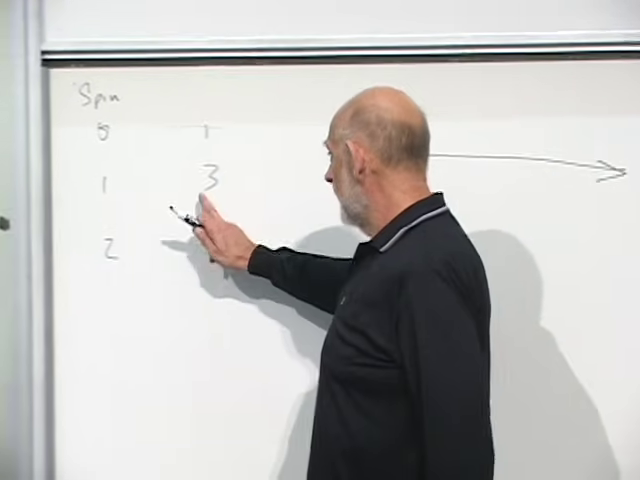
\includegraphics[width=\textwidth]{lecture_03_figure_07.png}
    \par\smallskip\footnotesize (a) 黑板上开始的自旋态计数。
  \end{minipage}\hfill
  \begin{minipage}[t]{0.5\textwidth}
    \centering
    \begin{adjustbox}{max width=\linewidth}
    \begin{tabular}{@{}ccc@{}}
      \toprule
      自旋 & 有质量态 & 无质量螺旋度 \\
      \midrule
      \(0\) & \(1\) & \(0\) \\
      \(1\) & \(3\) & \(+1,-1\) \\
      \(2\) & \(5\) & \(+2,-2\) \\
      \bottomrule
    \end{tabular}
    \end{adjustbox}
  \end{minipage}
  \caption{质量消除了静止系，也消除了中间的自旋投影。}
  \lectureframe{00:27:40}
  \label{fig:l03-spin-count}
\end{figure}

\subsection{线偏振与圆偏振光子}

取一个沿\(z\)运动的光子。它的两个横向线偏振是\(\ket{x}\)和\(\ket{y}\)。它们不是螺旋度本征态。圆偏振态是

\begin{align}
  \ket{R}
  &=\frac{1}{\sqrt2}\left(\ket{x}+i\ket{y}\right),
  \label{eq:l03-right-circular}\\
  \ket{L}
  &=\frac{1}{\sqrt2}\left(\ket{x}-i\ket{y}\right),
  \label{eq:l03-left-circular}
\end{align}

其螺旋度为\(+1\)和\(-1\)，取决于用来命名右旋和左旋的约定。线偏振光子是这两种结果的叠加。它的平均螺旋度可以为零，但螺旋度测量永远不会发现自旋为零的光子。同样，

\begin{equation}
  \frac{1}{\sqrt2}\left(\ket{x}+\ket{y}\right)
\end{equation}

就是四十五度方向的线偏振。

\begin{figure}[H]
  \centering
  \begin{minipage}[t]{0.48\textwidth}
    \centering
    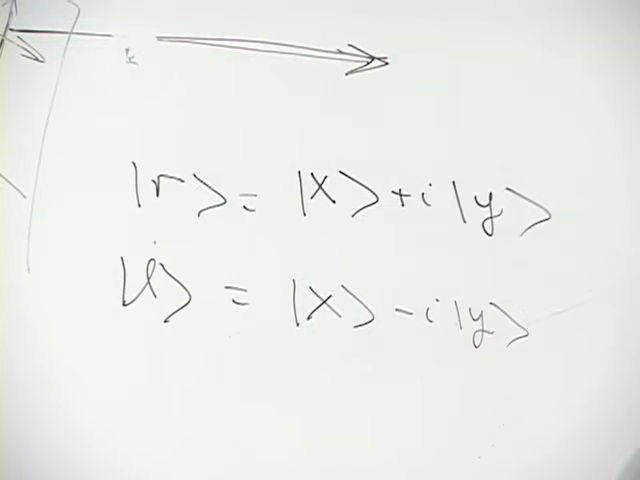
\includegraphics[width=\textwidth]{lecture_03_figure_08.png}
    \par\smallskip\footnotesize (a) 黑板上的圆偏振态。
  \end{minipage}\hfill
  \begin{minipage}[t]{0.48\textwidth}
    \centering
    \begin{adjustbox}{max width=\linewidth}
    \begin{tikzpicture}[>=Latex,scale=0.9]
      \draw[->,thick] (0,0) -- (3.4,0) node[right] {\(z\)};
      \draw[->,blue!70!black,thick] (0,0) -- (0,2.0)
        node[above] {\(x\)};
      \draw[->,orange!85!black,thick] (0,0) -- (-1.4,-1.2)
        node[below left] {\(y\)};
      \draw[red!70!black,thick,->]
        plot[domain=0:320,samples=80]
        ({1.0*cos(\x)},{0.58*sin(\x)+0.4});
      \node[red!70!black] at (1.55,1.25) {circular};
    \end{tikzpicture}
    \end{adjustbox}
  \end{minipage}
  \caption{线偏振提供横向基；圆偏振组合使螺旋度对角化。}
  \lectureframe{00:37:45}
  \label{fig:l03-polarization}
\end{figure}

\begin{classroomqa}
\audiencequestion{这是否类似于Stern--Gerlach实验中自旋态的分离？\lecturetimestamp{00:37:40}}
\lecturerresponse{量子叠加的想法是一样的，但对光子来说，直接的语言是偏振。圆偏振测量区分两个螺旋度；束流中不存在纵向的自旋为零的光子。}
\end{classroomqa}

引力子在自旋为2时重复了这一模式。为了进行自旋记账，可以示意性地写出

\begin{equation}
  \ket{+2}\sim\ket{+1}\otimes\ket{+1},
  \qquad
  \ket{-2}\sim\ket{-1}\otimes\ket{-1}.
  \label{eq:l03-graviton-helicity}
\end{equation}

这并不意味着引力子字面上由两个光子组成。它说的是两个相等的螺旋度相加得到正确的自旋为2的螺旋度。

\begin{classroomqa}
\audiencequestion{双光子类比是否推广到其他量子数？\lecturetimestamp{00:41:05}}
\lecturerresponse{不能作为组分模型。有一些强有力的公式，其中引力振幅看起来像规范理论振幅的乘积，或``平方，''但引力子仍然是它自己的粒子。这里的类比最可靠之处在于它是关于螺旋度的陈述。\editorialnote{现代Kawai--Lewellen--Tye关系和双拷贝关系在适当的理论中使振幅陈述变得精确；它们并不会把引力子变成两个光子的束缚态。}}
\end{classroomqa}

\begin{classroomqa}
\audiencequestion{光子可以具有任意动量，那么它难道不具有连续谱，而不是粒子所要求的孤立谱吗？\lecturetimestamp{00:42:17}}
\lecturerresponse{连续变量是质心动量。保持该动量固定，检查内部不变质量。粒子由孤立的质谱层来标识；改变其总动量则产生通常的连续色散关系。}
\end{classroomqa}

\section{最低的开弦能级}

现在我们可以回到弦。在大动量描述中，有限的内部光前能量正比于不变质量的平方。略去整体弦标度，将谱写成

\begin{equation}
  \begin{aligned}
    M^2
    &=m_0^2
      +\sum_{n=1}^{\infty}n
       \left(N_n^{(a)}+N_n^{(b)}\right),\\
    N_n^{(a)}&=a_n^\dagger a_n,
    \qquad
    N_n^{(b)}=b_n^\dagger b_n.
  \end{aligned}
  \label{eq:l03-open-spectrum}
\end{equation}

振子基态满足

\begin{equation}
  a_n\ket{0}=0,
  \qquad
  b_n\ket{0}=0,
  \qquad n=1,2,\ldots .
  \label{eq:l03-ground-annihilation}
\end{equation}

它并不是弦的空无缺席。它是最低激发的量子弦，其坐标仍然在涨落。设其质量平方为\(m_0^2\)，尚未确定。

\begin{figure}[H]
  \centering
  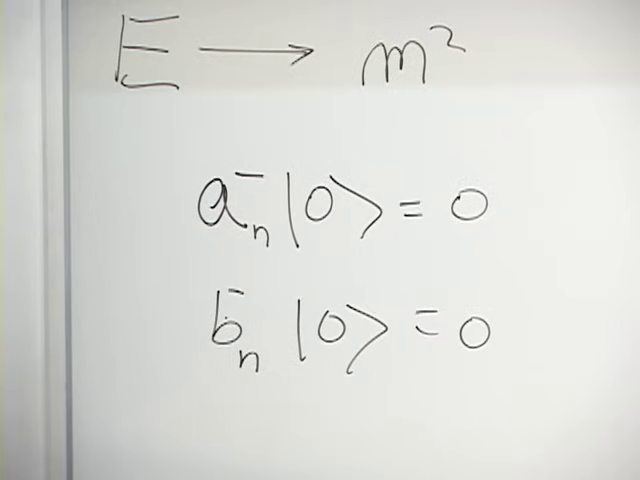
\includegraphics[width=0.78\textwidth]{lecture_03_figure_09.png}
  \caption{开弦基态以及定义它的湮灭条件。}
  \lectureframe{00:45:20}
  \label{fig:l03-ground-state-board}
\end{figure}

最廉价的激发使用\(n=1\)产生算符：

\begin{equation}
  a_1^\dagger\ket{0},
  \qquad
  b_1^\dagger\ket{0},
  \qquad
  M^2=m_0^2+1.
  \label{eq:l03-first-level}
\end{equation}

\begin{figure}[H]
  \centering
  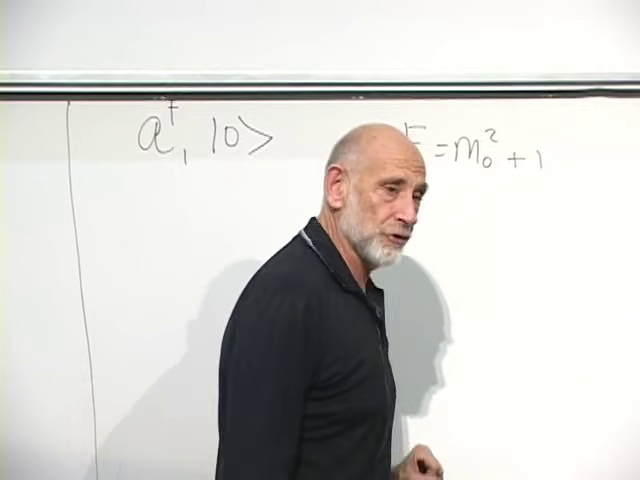
\includegraphics[width=0.78\textwidth]{lecture_03_figure_10.png}
  \caption{两个简并的第一能级态之一，黑板上写有其质量平方增量。}
  \lectureframe{00:49:25}
  \label{fig:l03-first-level-board}
\end{figure}

``一''在式{eq:l03-first-level}中不是一焦耳、一电子伏特，也不是一个普朗克质量。我们已经隐去了有量纲的弦标度。就目前而言，它指的是振子质量平方阶梯中的一步；缺失的单位将在下一讲中恢复。

这两个简并态的任何线性组合也是此能级上的一个态。特别地，

\begin{equation}
  \frac{1}{\sqrt2}
  \left(a_1^\dagger\pm i b_1^\dagger\right)\ket{0}
  \label{eq:l03-string-circular-states}
\end{equation}

是圆偏振的弦类比。在\(x\)-\(y\)平面中的旋转下，\(a_1^\dagger\)和\(b_1^\dagger\)的变换如同横向矢量的两个分量。因此\eqref{eq:l03-string-circular-states}中的组合具有螺旋度\(+1\)和\(-1\)。

\begin{figure}[H]
  \centering
  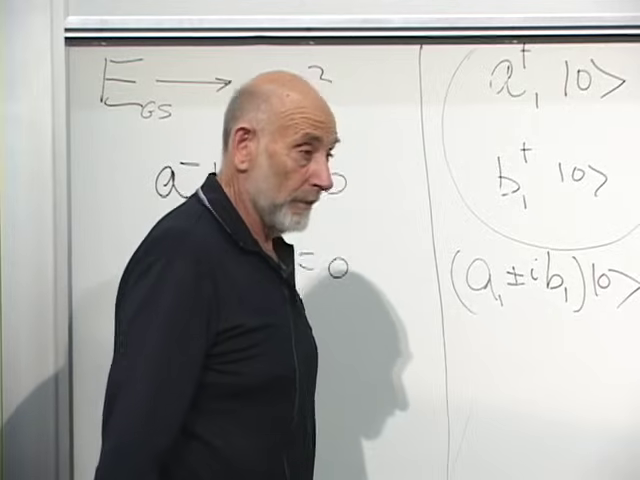
\includegraphics[width=0.82\textwidth]{lecture_03_figure_11.png}
  \caption{黑板上汇集了基态条件、两个第一能级激发及其圆组合。}
  \lectureframe{00:56:00}
  \label{fig:l03-level-structure-board}
\end{figure}

不存在可作为纵向偏振的第三个简并态。如果这两个态具有非零质量，自旋为一的相对论性粒子将需要三种偏振。恰好只有两种，该态就必须是无质量的。因此

\begin{equation}
  m_0^2+1=0,
  \qquad
  m_0^2=-1.
  \label{eq:l03-intercept-condition}
\end{equation}

第一能级是类光子的：它是一个无质量规范矢量态。它不必是电磁学中的光子；其最终的规范身份取决于弦模型。其下方的基态具有负质量平方。那就是玻色开弦快子。\editorialnote{在完整临界玻色弦中，正规序截距和洛伦兹代数与\(D=26\)相联系。本讲中两个横向方向的计算是同一态计数论证的四维投影：\(D-2\)个第一能级振子态与无质量矢量的\(D-2\)个物理偏振相匹配。}

\begin{classroomqa}
\audiencequestion{我们为什么应当关心\(m_0^2\)为负？\lecturetimestamp{00:56:35}}
\lecturerresponse{因为质量平方是二次场势关于我们称为真空的态的曲率。负曲率意味着该构型不是稳定的基态。接下来的计算将使这一陈述变得精确。}
\end{classroomqa}

\section{快子真正意味着什么}

``快子''这一名称会招致一种误导性的第一想法。从\(c=1\)的相对论色散关系出发，

\begin{equation}
  E(p)=\sqrt{p^2+m^2}.
  \label{eq:l03-relativistic-dispersion}
\end{equation}

对于波包，群速度为

\begin{equation}
  v_g=\frac{dE}{dp}.
  \label{eq:l03-group-velocity}
\end{equation}

这重现了熟悉的情形：

\begin{align}
  E_{\rm nr}(p)&=\frac{p^2}{2m},
  &v_g&=\frac{p}{m},
  \label{eq:l03-nr-group-velocity}\\
  E_\gamma(p)&=|p|,
  &|v_g|&=1,
  \label{eq:l03-photon-group-velocity}\\
  E_m(p)&=\sqrt{p^2+m^2},
  &|v_g|&=\frac{|p|}{\sqrt{p^2+m^2}}<1.
  \label{eq:l03-massive-group-velocity}
\end{align}

\begin{figure}[H]
  \centering
  \begin{minipage}[t]{0.48\textwidth}
    \centering
    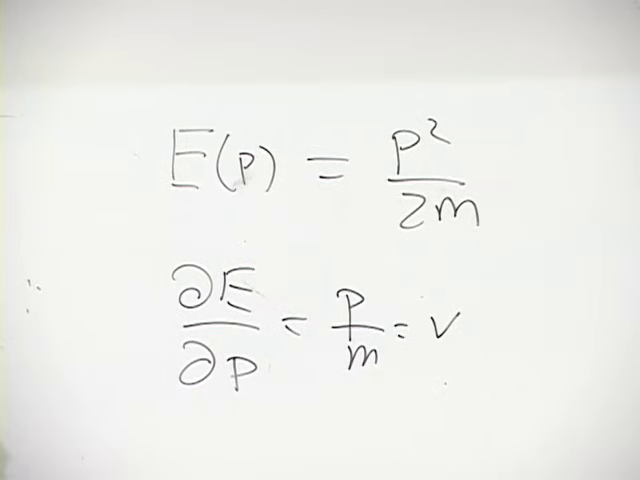
\includegraphics[width=\textwidth]{lecture_03_figure_12.png}
    \par\smallskip\footnotesize (a) 非相对论群速度。
  \end{minipage}\hfill
  \begin{minipage}[t]{0.48\textwidth}
    \centering
    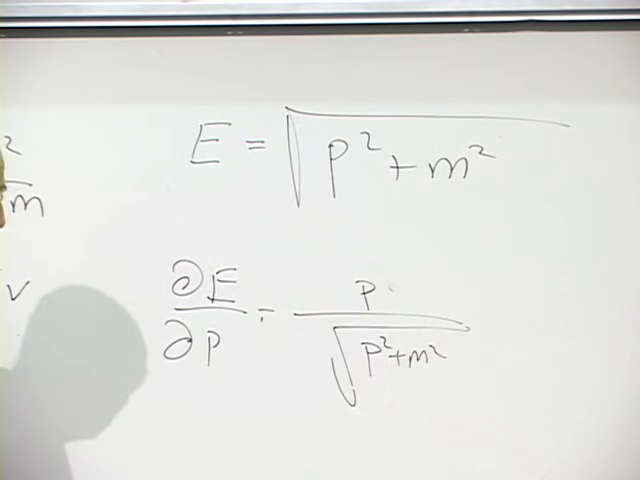
\includegraphics[width=\textwidth]{lecture_03_figure_13.png}
    \par\smallskip\footnotesize (b) 相对论色散及其
    导数。
  \end{minipage}
  \caption{从\(E(p)\)的斜率读取传播速率。}
  \lectureframe{01:01:50 and 01:03:15}
  \label{fig:l03-group-velocity-board}
\end{figure}

如果\(m^2=-\mu^2\)，形式表达式变为

\begin{equation}
  E(p)=\sqrt{p^2-\mu^2},
  \qquad
  v_g=\frac{p}{\sqrt{p^2-\mu^2}},
  \label{eq:l03-formal-tachyon-dispersion}
\end{equation}

只要平方根为实数，它就有\(|v_g|>1\)。但这不是玻色弦基态的正确物理解释。问题在低动量处就已经出现，那里频率是虚的。

\subsection{场势的负曲率}

考虑一维空间中的实标量场，

\begin{equation}
  \left(\partial_t^2-\partial_x^2+m^2\right)\phi=0.
  \label{eq:l03-klein-gordon}
\end{equation}

对于平面波\(\phi\propto e^{-i\omega t+ikx}\)，

\begin{equation}
  \omega^2=k^2+m^2.
  \label{eq:l03-kg-dispersion}
\end{equation}

\begin{figure}[H]
  \centering
  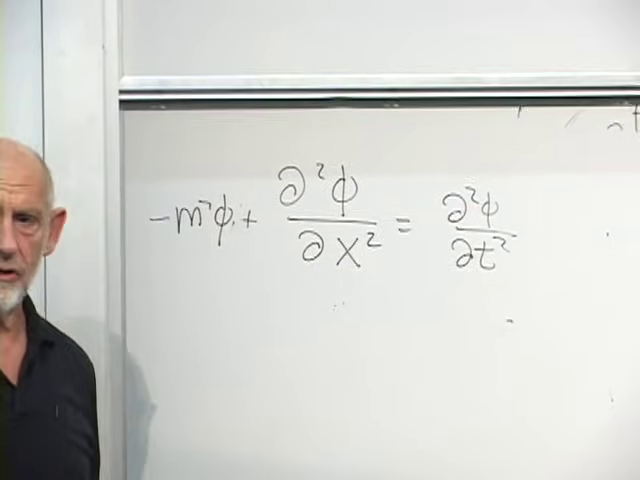
\includegraphics[width=0.82\textwidth]{lecture_03_figure_14.png}
  \caption{用于揭示负质量平方背后不稳定性的Klein--Gordon方程。}
  \lectureframe{01:06:40}
  \label{fig:l03-klein-gordon-board}
\end{figure}

守恒的二次能量为

\begin{equation}
  \mathcal E
  =\frac12\int dx\,
  \left[
    \dot\phi^{\,2}
    +(\partial_x\phi)^2
    +m^2\phi^2
  \right].
  \label{eq:l03-field-energy}
\end{equation}

\begin{figure}[H]
  \centering
  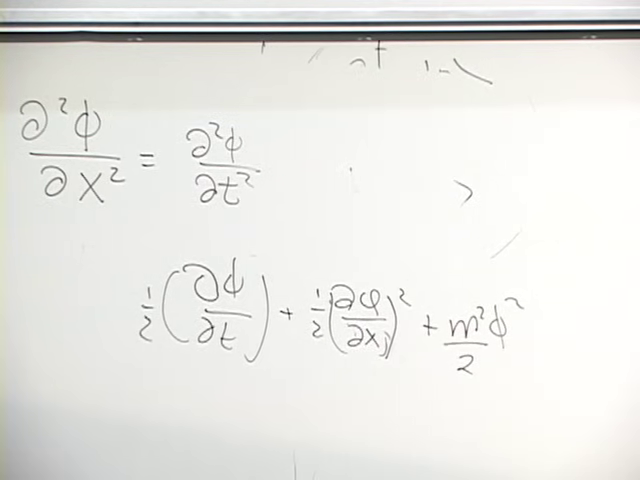
\includegraphics[width=0.82\textwidth]{lecture_03_figure_15.png}
  \caption{标量场能量，其中质量项提供势的局部曲率。}
  \lectureframe{01:08:10}
  \label{fig:l03-field-energy-board}
\end{figure}

对于\(m^2>0\)，局部势\(V(\phi)=\tfrac12m^2\phi^2\)是一个碗。构型\(\phi=0\)位于其底部。对于\(m^2=-\mu^2\)，同一点是倒置碗的顶部。方程\eqref{eq:l03-kg-dispersion}变为

\begin{equation}
  \omega^2=k^2-\mu^2.
  \label{eq:l03-tachyonic-modes}
\end{equation}

具有\(k^2<\mu^2\)的模有

\begin{equation}
  \omega=\pm i\sqrt{\mu^2-k^2},
  \qquad
  \phi_k(t)\propto
  e^{\pm\sqrt{\mu^2-k^2}\,t}.
  \label{eq:l03-growing-mode}
\end{equation}

一个分支指数增长。因此所谓的真空是不稳定的：任意小的长波扰动都会驱使场离开\(\phi=0\)。这就是谱中存在快子的含义。

\subsection{倒立摆链}

一排耦合摆使这一区别变得可见。让每个摆都竖直向上。均匀构型存在，但它平衡在势能的极大值处。轻推一个摆，它就会倒下，并拉动它的邻居。一个倒下的摆形成的前沿以由耦合固定的有限信号速度在链中传播。

\begin{figure}[H]
  \centering
  \begin{minipage}[t]{0.48\textwidth}
    \centering
    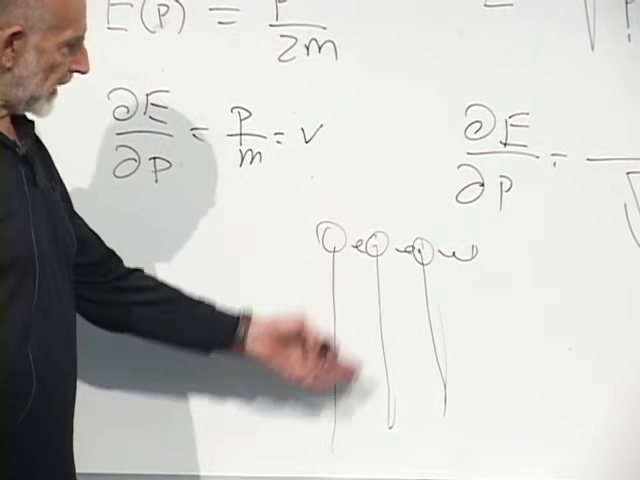
\includegraphics[width=\textwidth]{lecture_03_figure_16.png}
    \par\smallskip\footnotesize (a) 黑板上的耦合竖直摆模型。
  \end{minipage}\hfill
  \begin{minipage}[t]{0.48\textwidth}
    \centering
    \begin{adjustbox}{max width=\linewidth}
    \begin{tikzpicture}[>=Latex,scale=0.78]
      \draw[thick] (-0.3,0) -- (6.3,0);
      \foreach \x/\a in {0/0,1/0,2/8,3/28,4/55,5/72,6/78}{
        \fill (\x,0) circle (0.06);
        \draw[thick] (\x,0) -- ++({90-\a}:1.25);
        \fill[blue!65!black]
          ($(\x,0)+({90-\a}:1.25)$) circle (0.11);
      }
      \draw[red!70!black,->,thick] (1.7,-0.45) -- (4.6,-0.45)
        node[midway,below] {falling front};
    \end{tikzpicture}
    \end{adjustbox}
  \end{minipage}
  \caption{不稳定性在一个系统中以因果方式传播，即使其线性化谱包含负质量平方。}
  \lectureframe{01:10:40}
  \label{fig:l03-pendulum-instability}
\end{figure}

这一机制中没有任何东西允许受控信号超过因果前沿。快子模式诊断的是一个糟糕的展开点，而不是一个稳定的超光速信使。\editorialnote{对于局部相对论性场方程，前沿速度仍然是因果速度。实的高-\(k\)支的形式群速度并不会把不稳定真空变成超光速通信通道。}

\begin{classroomqa}
\audiencequestion{刚刚发现的无质量态就是弦理论预言的引力子吗？\lecturetimestamp{01:14:27}}
\lecturerresponse{不是。它是开弦的双极化自旋一态，因此类似规范玻色子。引力子是闭弦的自旋二激发。}
\end{classroomqa}

\begin{classroomqa}
\audiencequestion{倒置的势在数学上允许吗？系统在落下之后会在哪里结束？\lecturetimestamp{01:15:17}}
\lecturerresponse{它是一个完全合法的局部近似，但仅凭它自身没有基态，因为能量无下界。更完整的势可能再次向上弯折并拥有一个更低的极小值。系统随后会滚向或凝聚到那个稳定构型。}
\end{classroomqa}

普通的玻色弦恰好具有这一缺陷。它的更高振子态仍然是谱的一部分，但它们是不稳定背景的激发。自洽的超弦理论在其稳定扇区中移除开弦快子，同时保留无质量和有质量的弦激发。

\begin{classroomqa}
\audiencequestion{开弦态的其他性质是否也像它的两个极化那样与光子相符？\lecturetimestamp{01:17:07}}
\lecturerresponse{该态的行为如同无质量规范玻色子。它的详细电荷分配、辐射规则和身份取决于弦模型，因此应当称它类光子，而不是立即把它等同于电磁作用。那些相互作用性质将在后面展开。}
\end{classroomqa}

\section{弦如何相互作用}

自由谱只是理论的一半。弦也会结合和分裂。首先记住，一个激发的自由弦可以携带角动量是有用的。一根直的旋转弦绕其质心转动，它的能量和角动量沿着熟悉的弦轨迹一起上升。

\begin{figure}[H]
  \centering
  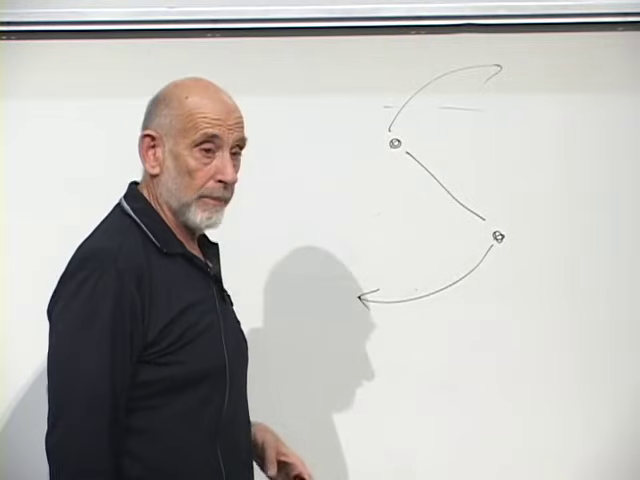
\includegraphics[width=0.72\textwidth]{lecture_03_figure_17.png}
  \caption{一根绕其质心点旋转的开弦的示意图。}
  \lectureframe{01:19:30}
  \label{fig:l03-rotating-string-board}
\end{figure}

\begin{classroomqa}
\audiencequestion{一根自由弦能绕一个固定端点翻转旋转吗？\lecturetimestamp{01:20:02}}
\lecturerresponse{没有锚点就不行。一个自由的孤立系统绕其质心旋转。如果一个端点附着在另一个物体或一个膜上，那么组合系统可以绕一个不同的中心旋转，正如电子和原子核绕它们的共同质心运动，而重得多的原子核看起来几乎固定。}
\end{classroomqa}

\subsection{开弦顶点}

对于开弦，基本相互作用发生在两个端点在同一时空点相遇时。它们结合并形成一根弦的振幅为 \(g_s\)。反转这一历史就给出了一根弦分裂成两根的振幅。示意地，

\begin{equation}
  \text{open}+\text{open}
  \quad\rightleftarrows\quad
  \text{open}.
  \label{eq:l03-open-joining}
\end{equation}

\begin{figure}[H]
  \centering
  \begin{minipage}[t]{0.48\textwidth}
    \centering
    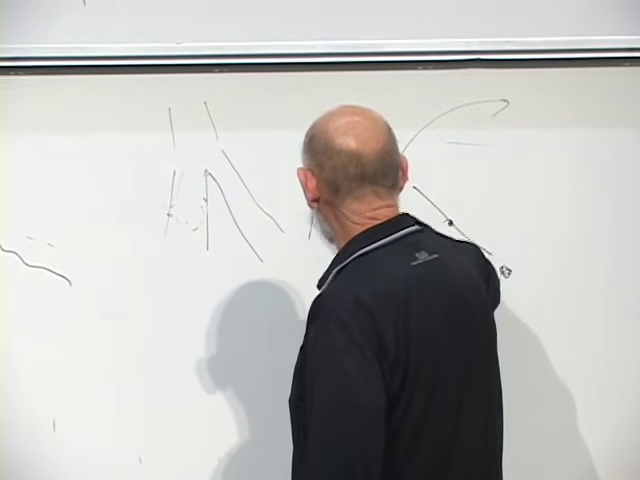
\includegraphics[width=\textwidth]{lecture_03_figure_18.png}
    \par\smallskip\footnotesize (a) 黑板上的结合历史。
  \end{minipage}\hfill
  \begin{minipage}[t]{0.48\textwidth}
    \centering
    \begin{tikzpicture}[>=Latex,scale=0.9]
      \draw[->] (0,-2.1) -- (0,2.2) node[above] {time};
      \draw[blue!70!black,thick] (-2,-1.6) .. controls (-1.3,-0.9)
        and (-0.7,-0.35) .. (0,0);
      \draw[blue!70!black,thick] (2,-1.6) .. controls (1.3,-0.9)
        and (0.7,-0.35) .. (0,0);
      \draw[orange!85!black,thick] (0,0) .. controls (0.25,0.7)
        and (-0.15,1.25) .. (0.15,1.9);
      \fill[red!70!black] (0,0) circle (0.09);
      \node[right] at (0.12,0) {\(g_s\)};
    \end{tikzpicture}
  \end{minipage}
  \caption{端点结合是局部粒子相互作用顶点的弦类似物；时间反演给出分裂。}
  \lectureframe{01:24:05}
  \label{fig:l03-open-vertex}
\end{figure}

耦合是一个振幅。对于一个指定的基本过程，相应的概率从 \(|g_s|^2\) 阶开始，相空间和归一化因子由完整计算提供。因此，把 \(g_s\) 称为 ``概率'' 是非正式的简写；保持振幅与概率的区分可以防止一个虚假的平方。

这种相互作用并不取决于外部弦恰好是在振动、旋转，还是处于某种其他的振子态。那些态会改变具体的矩阵元，但所用的仍是同一条局部连接规则。

\subsection{开弦可以自身闭合}

假设一条开弦的两个端点相遇。连接规则无法知道它们属于同一条弦。它们可以融合，产生一个闭合圈：

\begin{equation}
  \text{open}\longrightarrow\text{closed}.
  \label{eq:l03-self-closing}
\end{equation}

\begin{figure}[H]
  \centering
  \begin{minipage}[t]{0.48\textwidth}
    \centering
    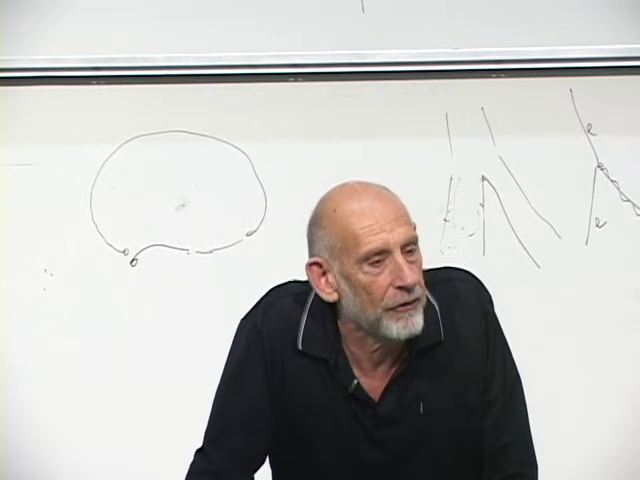
\includegraphics[width=\textwidth]{lecture_03_figure_19.png}
    \par\smallskip\footnotesize (a) 开弦把它的两个端点带到一起。
  \end{minipage}\hfill
  \begin{minipage}[t]{0.48\textwidth}
    \centering
    \begin{tikzpicture}[>=Latex,scale=0.92]
      \draw[blue!70!black,thick]
        (-2,0) .. controls (-1.2,1.5) and (1.2,1.5) .. (2,0);
      \fill[red!70!black] (-2,0) circle (0.08);
      \fill[red!70!black] (2,0) circle (0.08);
      \draw[->,thick] (-0.45,-0.45) -- (0.45,-0.45);
      \draw[orange!85!black,thick] (0,-1.55) ellipse (1.15 and 0.58);
      \node at (0,-2.25) {closed string};
    \end{tikzpicture}
  \end{minipage}
  \caption{相互作用的开弦不可避免地会产生闭弦。}
  \lectureframe{01:27:20}
  \label{fig:l03-open-becomes-closed}
\end{figure}

这不是可有可无的装饰。任何关于相互作用开弦的理论都必须包含闭弦态。逆过程则允许闭弦在存在允许的端点和边界条件时打开成一条开弦。

\begin{classroomqa}
\audiencequestion{当弦融合或分裂时，它们的振子能量会改变吗，理论是否决定了如何改变？\lecturetimestamp{01:28:05}}
\lecturerresponse{会。对于整个过程，能量和动量守恒，而激发可以在出射弦之间重新分配。相互作用顶点和外部波函数决定跃迁振幅。}
\end{classroomqa}

\subsection{闭弦可以在不打开的情况下相互作用}

这一蕴含关系是单向的。相互作用的开弦需要闭弦，但一个理论可以只从闭弦开始。两个闭合圈可以接触、重新连接，并变成一个闭合圈；相反的历史则把一个圈分裂成两个。无需出现任何开端点。

\begin{figure}[H]
  \centering
  \begin{minipage}[t]{0.48\textwidth}
    \centering
    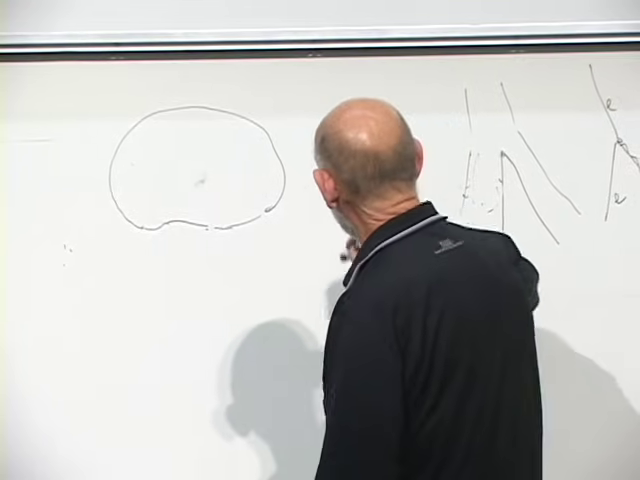
\includegraphics[width=\textwidth]{lecture_03_figure_20.png}
    \par\smallskip\footnotesize (a) 黑板上的闭弦融合。
  \end{minipage}\hfill
  \begin{minipage}[t]{0.48\textwidth}
    \centering
    \begin{tikzpicture}[>=Latex,scale=0.88]
      \draw[blue!70!black,thick] (-1.35,0) circle (0.75);
      \draw[blue!70!black,thick] (1.35,0) circle (0.75);
      \draw[->,thick] (-0.35,-1.15) -- (0.35,-1.15);
      \draw[orange!85!black,thick] (0,-2.3) ellipse (1.35 and 0.68);
      \node at (0,1.2) {closed \(+\) closed};
      \node at (0,-3.25) {closed};
    \end{tikzpicture}
  \end{minipage}
  \caption{闭弦拥有自己的连接与分裂相互作用，无需经过开弦态。}
  \lectureframe{01:29:05}
  \label{fig:l03-closed-fusion}
\end{figure}

\begin{classroomqa}
\audiencequestion{如果一个理论从闭弦开始，它是否也必须包含开弦？\lecturetimestamp{01:28:35}}
\lecturerresponse{不。闭弦可以通过重新连接而相互作用，同时始终保持闭合。开弦需要额外的边界数据，例如允许的端点或膜。}
\end{classroomqa}

\section{为什么引力无法避免}

闭弦振子的计算与开弦的类似，但存在独立的左行和右行激发。它们最低的非平凡匹配能级包含一个无质量的自旋二态。该态具有引力子的螺旋度。因此，每一个自洽的相互作用闭弦理论都包含引力。

\begin{classroomqa}
\audiencequestion{为什么最低的闭弦激发必须是引力子，正如开弦能级必须是类光子的那样？
\lecturetimestamp{01:30:59}}
\lecturerresponse{答案是同一种态计数，现在带有左行和右行振子矢量。它们的张量积包含一个无质量的对称无迹自旋二极化。显式的闭弦谱将在下一步算出；在现阶段，要点是那个态的不可避免性。}
\end{classroomqa}

开弦和闭弦也可以彼此相互作用。一个闭合圈可以遇到一条开弦并被吸收，留下一条更大或激发方式不同的开弦。反过来，一条开弦可以辐射出一个闭合圈。在粒子层面，这就是物质对引力子的发射或吸收。

\begin{figure}[H]
  \centering
  \begin{minipage}[t]{0.48\textwidth}
    \centering
    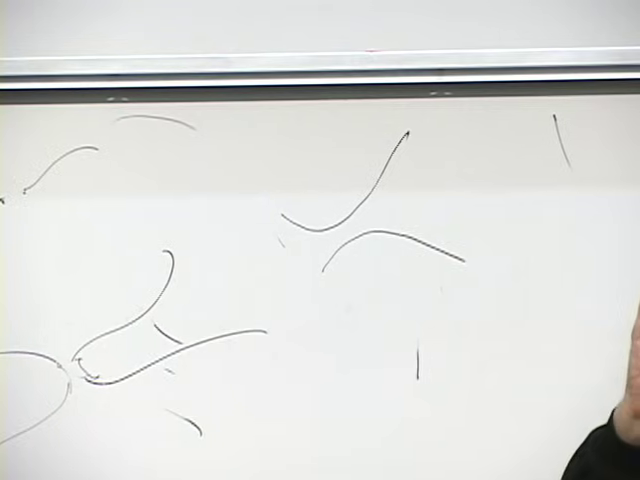
\includegraphics[width=\textwidth]{lecture_03_figure_21.png}
    \par\smallskip\footnotesize (a) 弦段的局部重新连接。
  \end{minipage}\hfill
  \begin{minipage}[t]{0.48\textwidth}
    \centering
    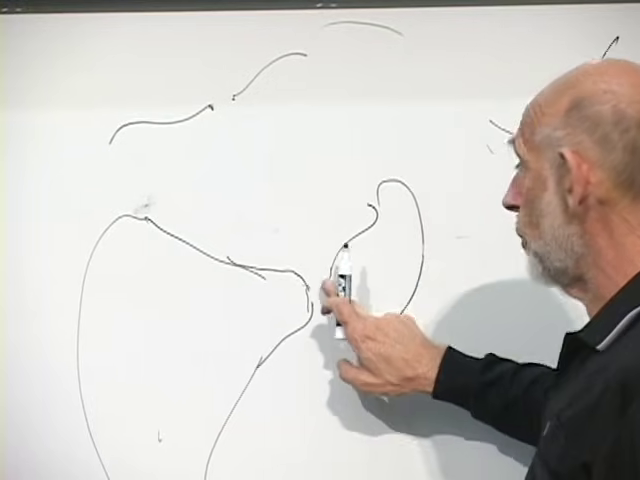
\includegraphics[width=\textwidth]{lecture_03_figure_22.png}
    \par\smallskip\footnotesize (b) 一个闭合圈附着到一条开弦上。
  \end{minipage}
  \caption{混合开--闭相互作用以及引力子交换的普遍可能性背后的黑板图景。
  }
  \lectureframe{01:33:10 and 01:34:35}
\label{fig:l03-mixed-interactions-board}
\end{figure}

\begin{figure}[H]
  \centering
  \begin{tikzpicture}[>=Latex,scale=0.88]
    \draw[blue!70!black,thick]
      (-3,-0.5) .. controls (-1.7,-0.1) and (-0.8,0.2) .. (0,0);
    \draw[blue!70!black,thick]
      (0,0) .. controls (0.9,0.3) and (2.0,0.1) .. (3,0.55);
    \draw[orange!85!black,thick] (-0.8,1.55) ellipse (0.75 and 0.45);
    \draw[->,red!70!black,thick] (-0.45,1.15) -- (-0.05,0.35);
    \node[blue!70!black] at (-2.2,-0.95) {open string};
    \node[orange!85!black] at (-0.8,2.25) {closed string};
    \node at (1.75,-0.5) {excited open string};
  \end{tikzpicture}
  \caption{一幅干净的、不依赖时空的闭弦被开弦吸收的示意图。}
  \label{fig:l03-mixed-interaction-redraw}
\end{figure}

引力子可以耦合到每一种弦态，因为每条弦都携带能量和动量，而且连接规则允许闭弦交换。这就是引力普适性的弦论起源。

\begin{classroomqa}
\audiencequestion{闭弦能否变成开弦，或者能否在不违反端点规则的情况下与开弦结合？\lecturetimestamp{01:31:20}}
\lecturerresponse{在同时包含这两个部分的弦理论中，闭弦可以附着到开弦上并改变其状态。单独一根闭弦能否直接打开，取决于该理论是否提供了允许的端点。局域重联规则保持不变。}
\end{classroomqa}

\begin{classroomqa}
\audiencequestion{闭圈能否永久地相互链接或打结？\lecturetimestamp{01:35:10}}
\lecturerresponse{在弱耦合下弦基本上是透明的：除非很小的重联振幅起作用，它们可以相互穿过。因此链接或结可以在一段时间内持续存在，但当允许的弦相互作用发生时，拓扑可以改变。}
\end{classroomqa}

\begin{classroomqa}
\audiencequestion{相互作用概率是否与弦的状态或速率无关？\lecturetimestamp{01:36:09}}
\lecturerresponse{局域耦合是同一个参数，但总跃迁概率还取决于波函数以及相关部分保持接触的时间长短。快速的相遇通常比缓慢的相遇提供更少的相互作用时间。}
\end{classroomqa}

\section{仍然缺失的标度和耦合}

有两笔账被有意推迟了。第一，\(X\) 是长度，而 \(a_n\) 是无量纲的，因此 \eqref{eq:l03-mode-coordinates} 中的比例关系必须包含一个长度标度。第二，提高振子能级不可能真的把一个无量纲数加到物理质量的平方上。恢复弦长 \(\ell_s\)，或等价地恢复 Regge 斜率 \(\alpha'\sim\ell_s^2\)，就补上了缺失的量纲：

\begin{equation}
  M^2\sim\frac{1}{\alpha'}(N-a).
  \label{eq:l03-dimensional-spectrum}
\end{equation}

精确的约定和归一化将在下一讲中确定。

\begin{classroomqa}
\audiencequestion{是什么确定了弦长的单位和单个产生算符所增加的质量？\lecturetimestamp{01:37:03}}
\lecturerresponse{一个带量纲的常数被省略了。它就是弦标度，通常写作 \(\ell_s\) 或 \(\alpha'\)。振子算符是无量纲的；该标度的幂次把它们的能级数转换为物理长度、张力和质量平方。}
\end{classroomqa}

第二个参数是弦耦合 \(g_s\)。在最简单的讨论中，它是一个控制结合与分裂的普适数。在更丰富的模型中，端点可以携带不同的标记，弦可以在交汇处相遇。Y 形构型是三条通量管相遇的弦类比；在旧强子图像中，它与三夸克重子相关联，而单个开弦段则类似于夸克--反夸克介子。

\begin{classroomqa}
\audiencequestion{不同的弦端点能否具有不同的结合概率？\lecturetimestamp{01:39:31}}
\lecturerresponse{最简单的模型使用一个耦合。更精细的理论把荷或边界标记附着到端点上，然后由选择定则决定哪些结合是允许的。详细构造留待以后，但普适的局域结合思想仍然成立。}
\end{classroomqa}

\begin{classroomqa}
\audiencequestion{弦能否纵向分裂或形成 Y 形交汇？\lecturetimestamp{01:40:01}}
\lecturerresponse{某些弦系统确实允许交汇。它们不是刚才画出的普通双端点分裂过程，而是当理论具有相容的弦荷时才会出现。介子--重子通量管类比是理解这一区别的有用图像。}
\end{classroomqa}

\begin{classroomqa}
\audiencequestion{改变时空维数会改变相互作用耦合吗？\lecturetimestamp{01:42:25}}
\lecturerresponse{维数会改变谱、相空间以及紧致化后得到的有效耦合。基本弦耦合仍然组织微扰展开，但它在低维中的表现取决于额外维的几何和体积。}
\end{classroomqa}

\begin{classroomqa}
\audiencequestion{引力是自由弦一开始运动的原因吗？\lecturetimestamp{01:43:17}}
\lecturerresponse{维持运动不需要力。初始位置和速度指定了一个自由解；惯性使它继续前进。引力或其他力会改变这种运动。追问初始条件的成因是一个独立的问题，不属于局域运动方程的一部分。}
\end{classroomqa}

因此我们得到了三个相互关联的结论。对开弦进行量子化会在其第一激发能级产生一个无质量矢量；其下方的玻色子基态是不稳定的；而相互作用不可避免地引入闭弦，其谱中包含引力。接下来的任务是恢复缺失的标度，并明确地进行闭弦量子化。
